\FloatBarrier
\section{\review{Model Estimates}}
\label{sec:nl_chroma_model}


The model of the LHC is based on MADX and magnetic field error tables~\cite{p_hagen_wise_2006},
containing a hundred seeds for the random errors. To compute the chromaticity, simulations are run
via PTC, with selected field errors.
Field errors are applied to all magnets, with $b_2$ errors in the main dipoles generating a
$\beta$-beating of approximately $10\%$. Coupling is introduced using global knobs to create a $C^-$
value of $0.001$, which is commonly observed during operation.

% =================================
%\subsection{\review{Major contributions}}

Simulations with various field errors have been run to assess the contribution of individual magnet
order and combinations for the fourth and firth order chromaticity. Normal and skew fields errors
ranging from sextupolar ($b_3$) to decahexapolar ($b_8$) are added alone or in combination to
observe which is the strongest. Quadrupolar field errors ($b_2$) introduce beta-beating. Coupling is
introduced via skew quadrupolar correctors.


% ----------------------------------
\subsubsection{\review{Fourth Order Chromaticity}}

The results from simulations strongly imply that the dodecapolar errors are the main contributors
to $Q^{(4)}$, as can be seen in \cref{fig:high_orders:beam1_q4_ptc}.
The most notable effect on this chromaticity order is the beta-beating, introducing a very large
spread via the various error seeds.
Comparing the simulation at the top with most errors added, the $b_6$ component alone accounts for
$\approx 70\%$ of it for both axes on each beam.

\begin{figure}[!htb]
    \centering
    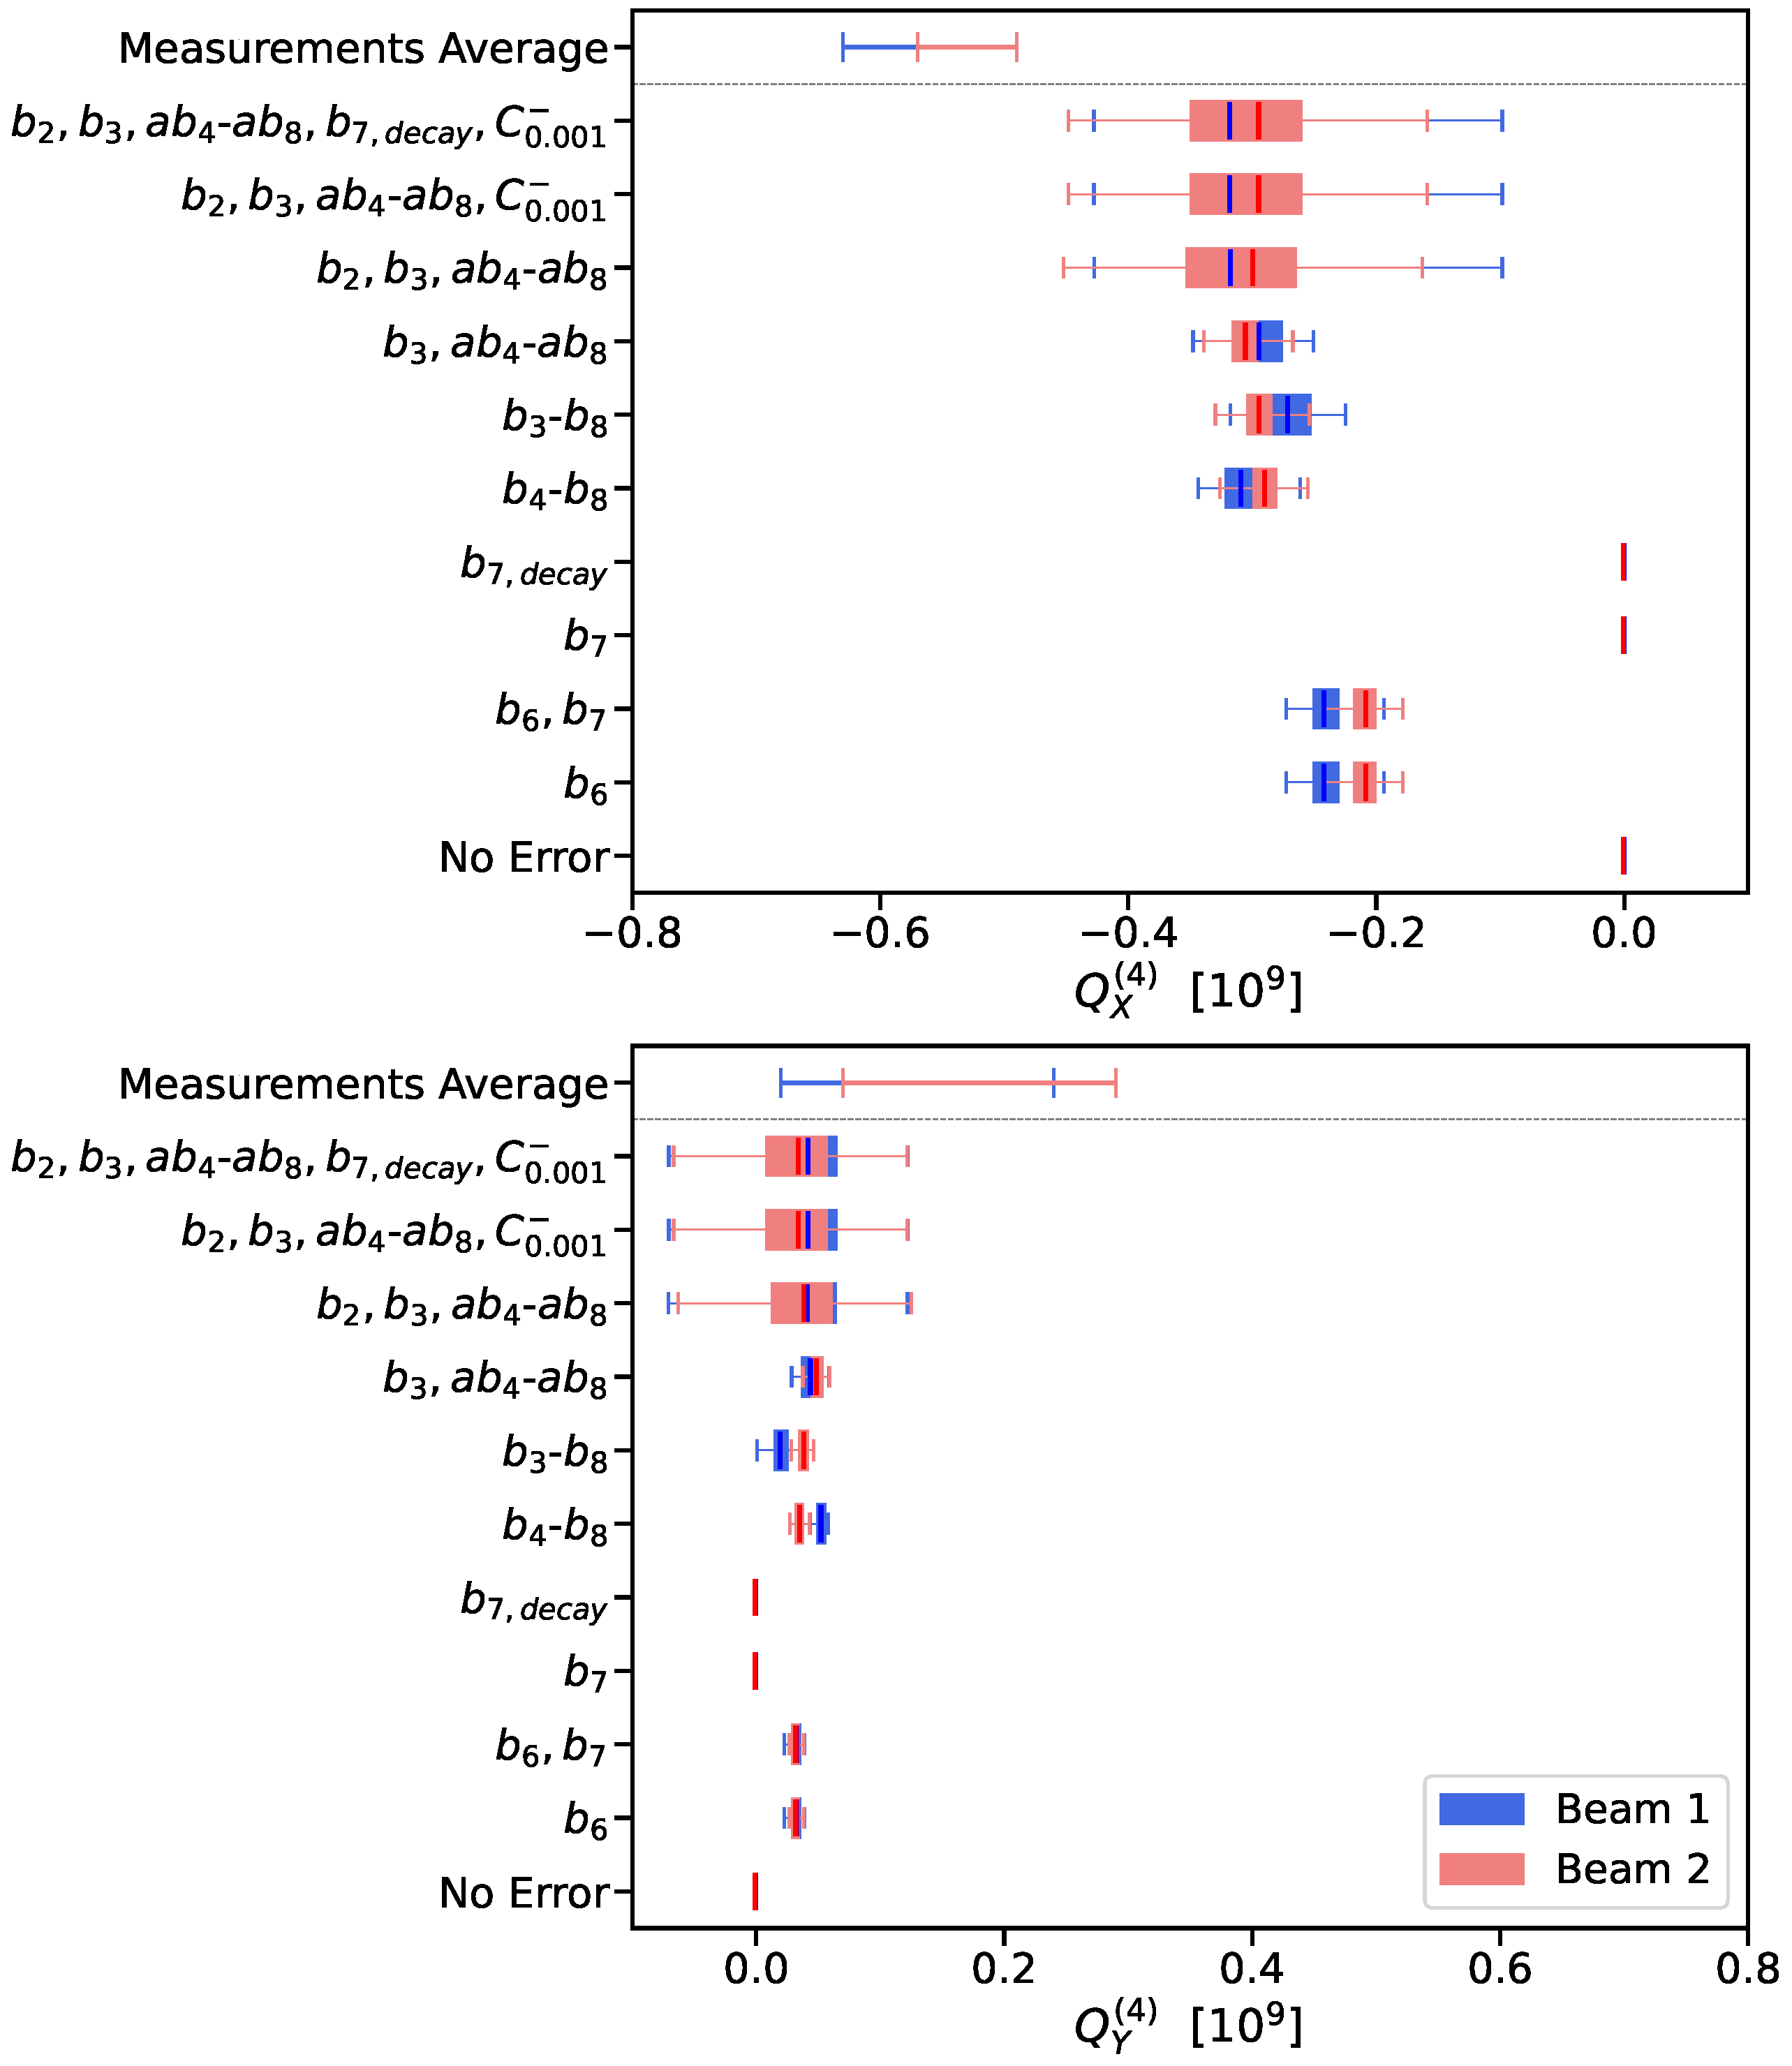
\includegraphics[width=0.9\columnwidth]{images/q4_ptc.pdf}
    \caption{Measured and simulated fourth order chromaticity with different multipole errors. The
    $b_2$ errors, applied on dipoles and quadrupoles, generate beta-beating. Coupling is set to a
    value commonly seen in operation.}
    \label{fig:high_orders:beam1_q4_ptc}
\end{figure}



% ----------------------------------
\FloatBarrier
\subsubsection{\review{Fifth Order Chromaticity}}

It is seen that the the decatetrapolar errors are the main contributors to $Q^{(5)}$, as can be seen
in \cref{fig:high_orders:beam1_q5_ptc}. Fringe fields and skew multipoles have been found to have a
negligible impact. 
Beta-beating and coupling are seen to increase by a small amount the chromaticity, while sextupolar
errors induce a spread with the different seeds. 
Comparing the simulation at the top with most errors added, the $b_7$ component alone accounts for
$\approx 70\%$ of it for both axes on each beam of the fifth order chromaticity.

\begin{figure}[!htb]
    \centering
    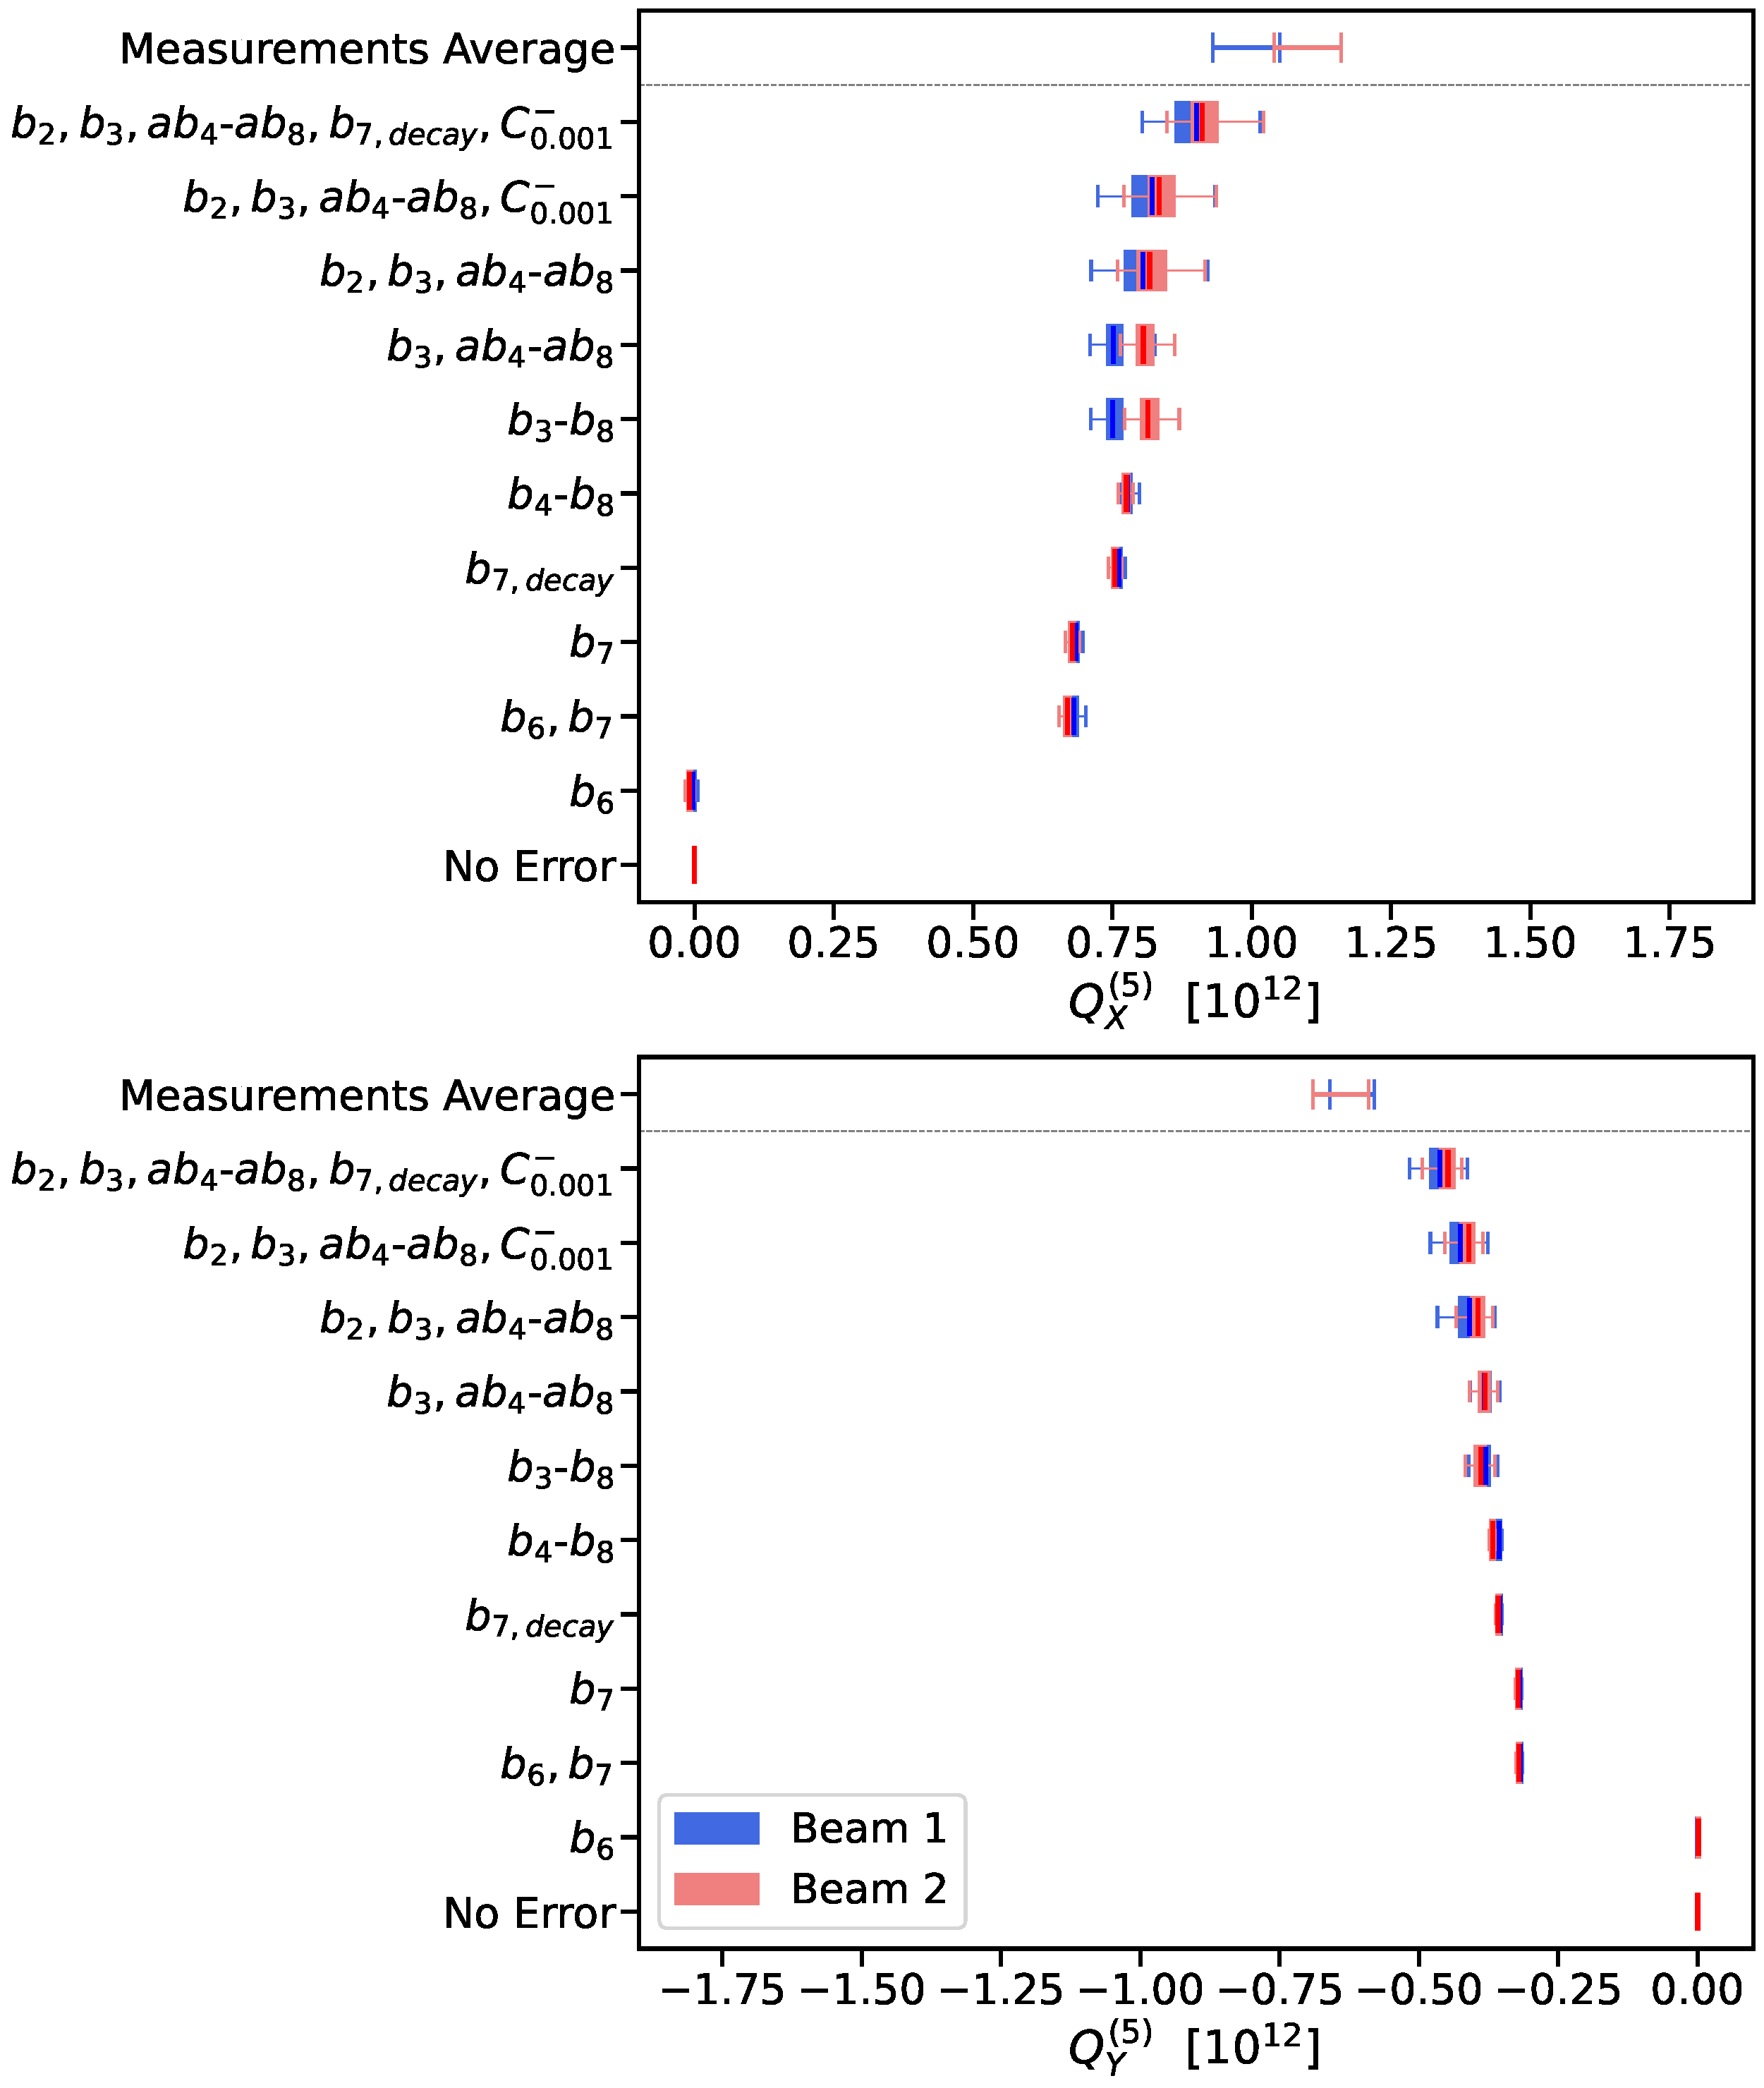
\includegraphics[width=0.9\columnwidth]{images/q5_ptc.pdf}
    \caption{Measured and simulated fifth order chromaticity with different multipole errors. The
    $b_2$ errors, applied on dipoles and quadrupoles, generate beta-beating. Coupling is set to a
    value commonly seen in operation.}
    \label{fig:high_orders:beam1_q5_ptc}
\end{figure}

%====================
%\subsection{\review{Decatetrapolar Decay}}

It has been noted in the previous chapter about decapoles (see \cref{section:decapoles:decay}) that
the $b_5$ component in the main dipoles was large at injection energy, and could explain most of the
discrepancy between the measurements and simulations.
Such a decay in the main dipoles also exists for the $b_7$ component~\cite{deniau2024private}, and
is shown in \cref{fig:high_orders:b7_decay}. 

\begin{figure}[!htb]
    \centering
    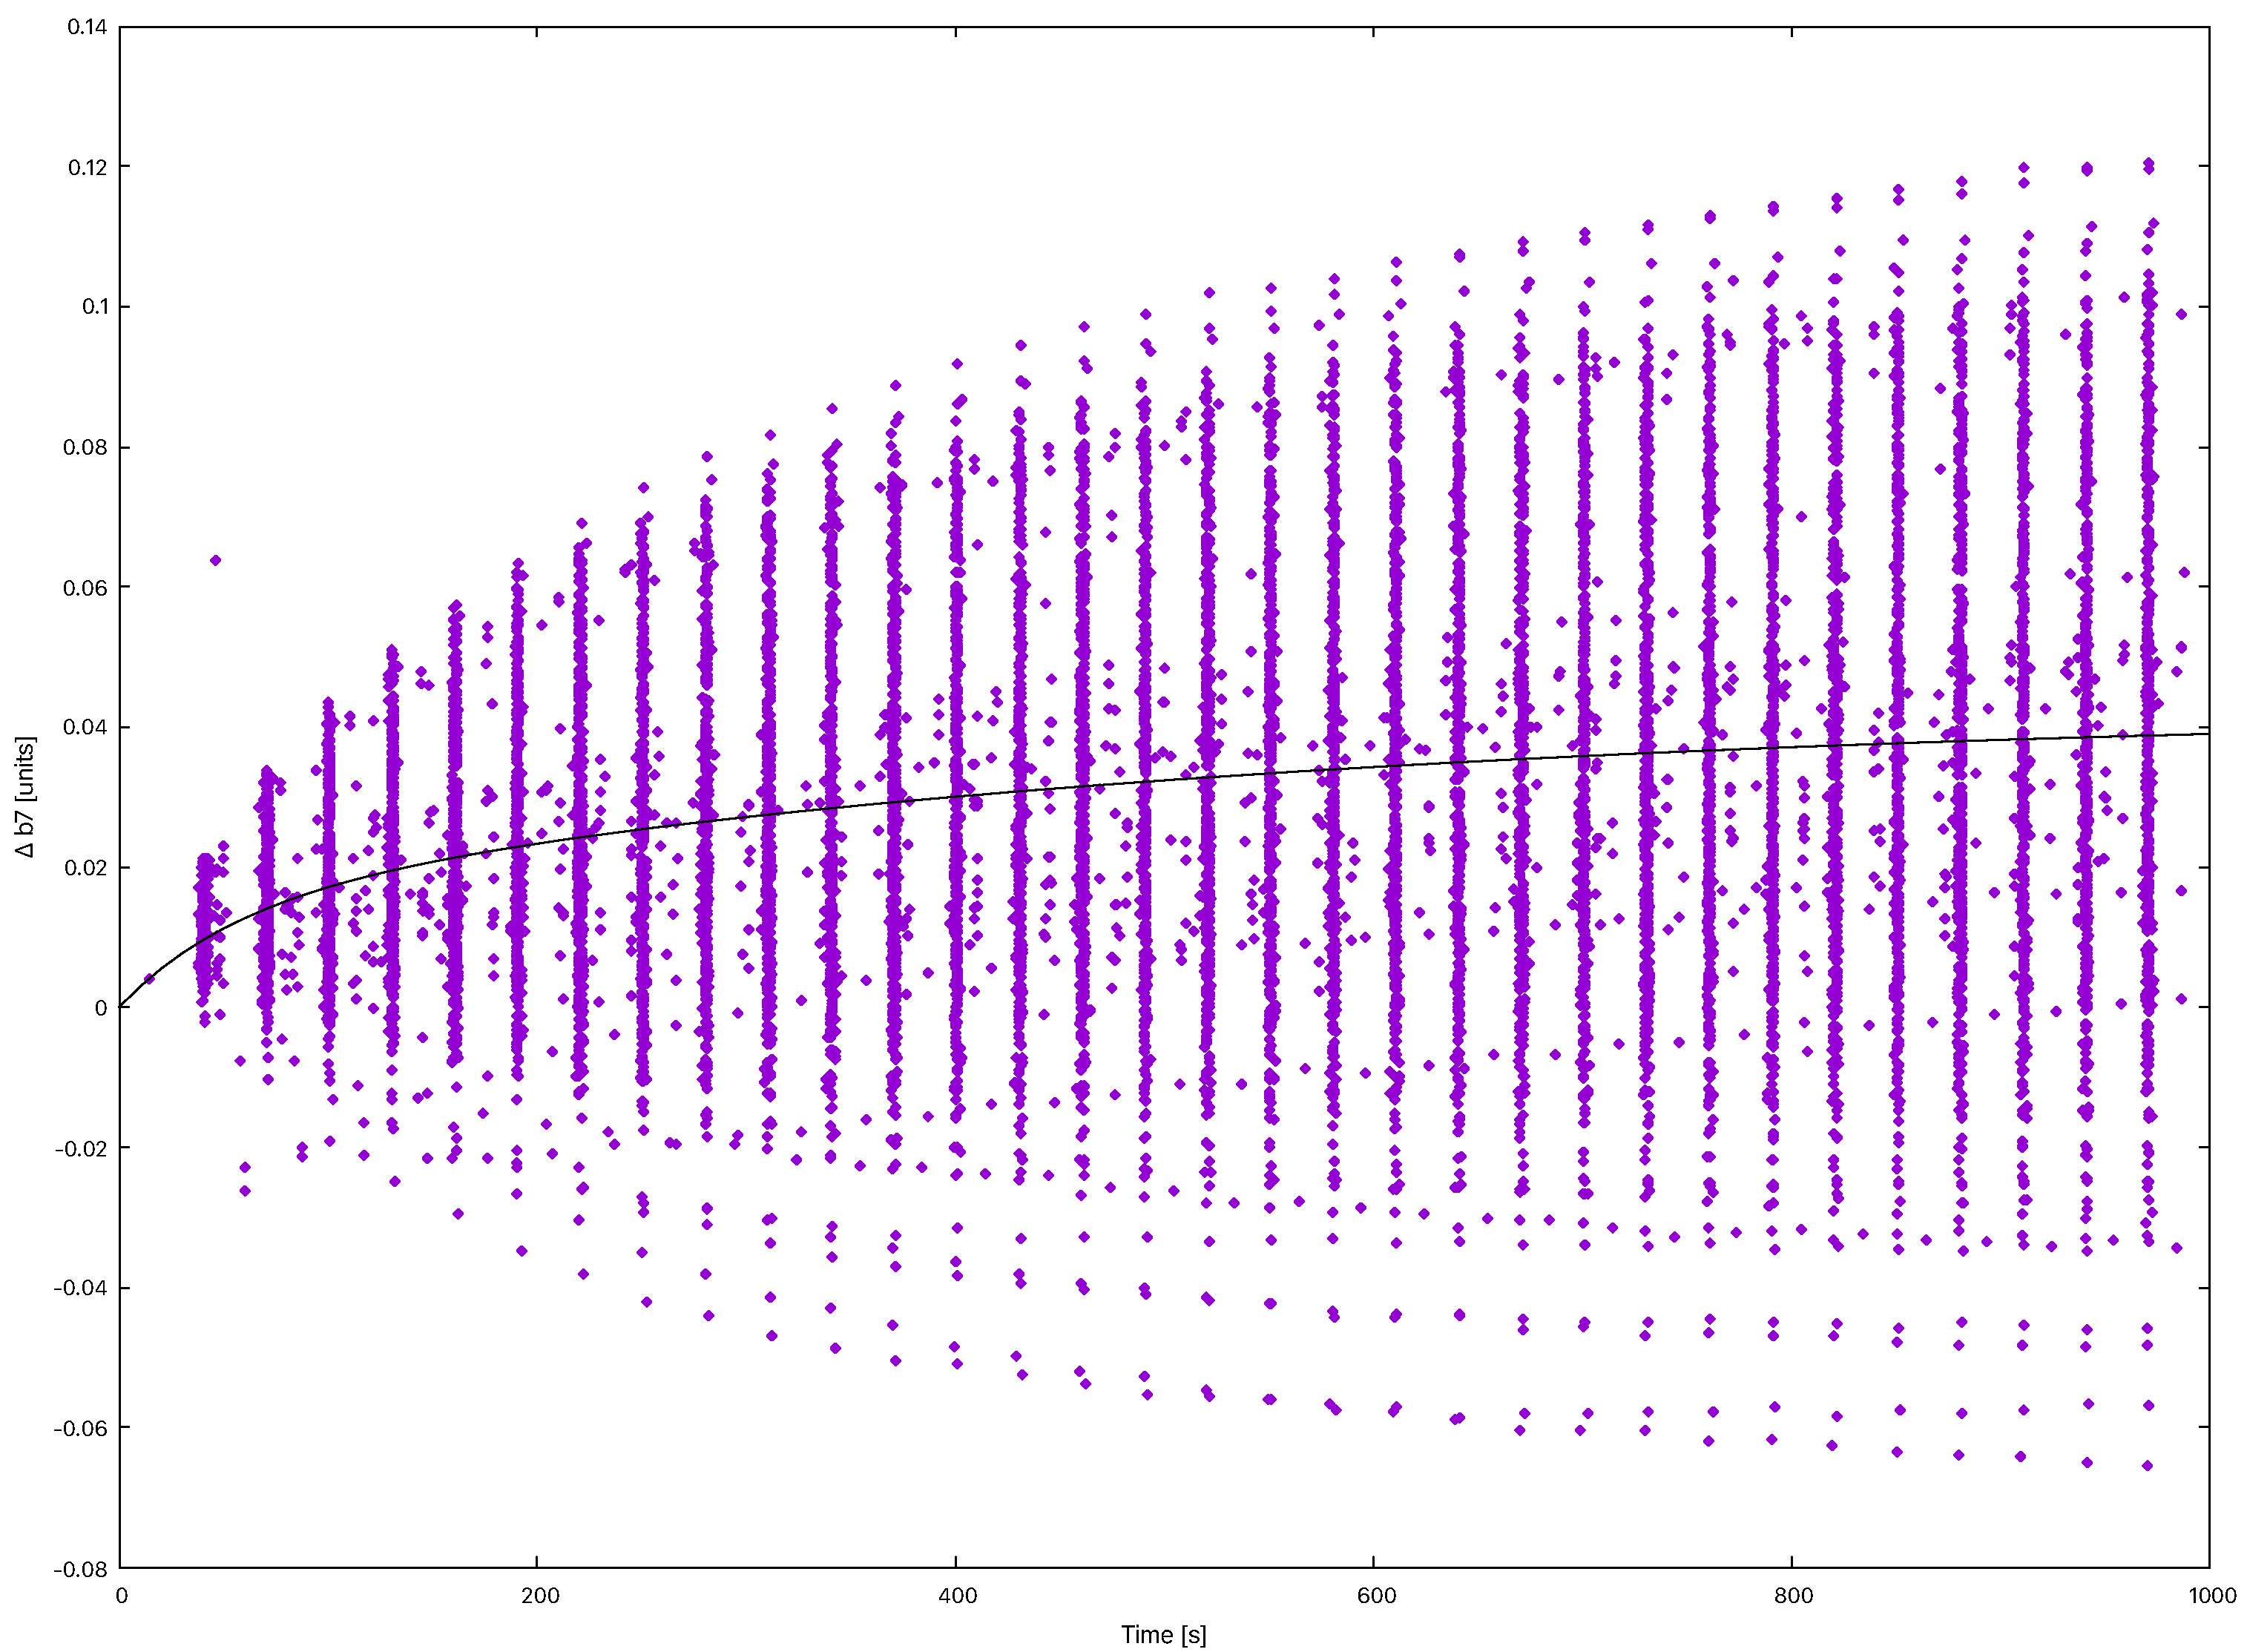
\includegraphics[width=0.9\columnwidth]{images/decay_b7.pdf}
    \caption{Measured decay of the integrated decatetrapolar field in LHC's main dipoles at
    injection energy. The fit is shown in black~\cite{deniau2024private} and settles around
    $+0.035$.}
    \label{fig:high_orders:b7_decay}
\end{figure}

Its value is though small and settles around $+0.0351 \pm 0.0007$. The average $b_7$ of the main
dipoles is of $0.32 \pm 0.16$. The decay thus increase that value of only about $11\%$.
Simulations done with that decay taken into account are also present in the previous
\cref{fig:high_orders:beam1_q5_ptc}.


% =================================
\FloatBarrier
\subsubsection{\review{Agreement with Measurements}}

Previous simulation results are shown in \cref{tab:high_orders:ptc_values}, taking the values from 
the simulation including the most effects at the top of the plots. For the fourth order, the beating
is not included as the large beating is not yet explained.
\Cref{tab:high_orders:ptc_values_ratios} shows the ratio between the measured average and simulated
chromaticities.

\begin{table}[!htb]
  \centering
  \begin{tabular}{lrr}
  \toprule
      Plane     &  $Q^{(4)} [10^9]$  &  $Q^{(5)} [10^{12}]$ \\
  \midrule
      Beam 1    &              &               \\
      \hspace{2mm}X         & $-0.29 \pm 0.02$ & $ 0.90 \pm 0.05$  \\
      \hspace{2mm}Y         & $ 0.04 \pm 0.01$ & $-0.46 \pm 0.03$  \\
      Beam 2    &  &   \\
      \hspace{2mm}X         & $-0.31 \pm 0.02$ & $ 0.92 \pm 0.03$ \\
      \hspace{2mm}Y         & $ 0.05 \pm 0.00$ & $-0.45 \pm 0.01$ \\
  \bottomrule
  \end{tabular}
  \caption{Simulated high order chromaticity terms via PTC at injection energy, including normal and
  skew sextupolar to decahexapolar field errors. Are also included beta-beating, coupling and
  decatetrapolar decay. For the fourth order, the values do not include beta-beating as the observed
  spread is not yet fully understood.}
  \label{tab:high_orders:ptc_values}
\end{table}

%\begin{table}[!htb]
%  \centering
%  \footnotesize
%  \begin{tabular}{lcccc}
%    \toprule
%                    &  \multicolumn{2}{c}{$Q^{(4)}$ Ratio}   &  \multicolumn{2}{c}{$Q^{(5)}$ Ratio} \\
%    \cmidrule(lr){2-3}\cmidrule(lr){4-5}
%      Plane         & First Meas.  & Second Meas.& First Meas.& Second Meas. \\ 
%    \midrule
%      Beam 1        &           &             &            & \\
%      \hspace{2mm}X &  $1.91\pm0.15$ & $2.15\pm0.17$    & $1.33\pm0.10$  & $1.35\pm0.09$   \\
%      \hspace{2mm}Y &  $3.50\pm0.90$ & $0.90\pm0.50$    & $1.91\pm0.22$  & $1.21\pm0.11$   \\
%      Beam 2        &                   &               &     & \\
%      \hspace{2mm}X &                & $4.90\pm1.00$    &                & $1.17\pm0.08$   \\
%      \hspace{2mm}Y &  $1.90\pm0.12$ & $3.30\pm0.50$    & $1.65\pm0.29$  & $1.47\pm0.12$   \\
%      \bottomrule
%  \end{tabular}
%  \caption{Ratios of the simulated and measured high order chromaticity terms for both the first and
%  second performed measurements. The values are taken from tables
%  \cref{tab:high_orders:chroma_fidel}, \cref{tab:high_orders:chroma_table_after} and
%  \cref{tab:high_orders:ptc_values}. The fit with high correlation between both terms is not
%  included.}
%  \label{tab:high_orders:ptc_values_ratios}
%\end{table}

\begin{table}[!htb]
    \centering
    \begin{tabular}{lcc}
      \toprule
        Plane         & $Q^{(4)}$ Ratio&  $Q^{(5)}$ Ratio \\
      \midrule
        Beam 1        &                &                  \\
        % Via weighted mean, which is probably not right.
        %\hspace{2mm}X &  $1.98\pm0.16$ & $1.10\pm0.09$    \\
        %\hspace{2mm}Y &  $3.00\pm0.70$ & $1.34\pm0.11$    \\
        \hspace{2mm}X &  $1.91\pm0.28$ & $1.24\pm0.23$    \\
        \hspace{2mm}Y &  $3.00\pm2.60$ & $1.47\pm0.27$    \\
        Beam 2        &                &                  \\
        %\hspace{2mm}X &  $1.74\pm0.11$ & $1.20\pm0.08$    \\
        %\hspace{2mm}Y &  $2.90\pm0.50$ & $1.42\pm0.12$    \\
        \hspace{2mm}X &  $1.74\pm0.16$ & $1.34\pm0.29$    \\
        \hspace{2mm}Y &  $3.70\pm2.30$ & $1.51\pm0.14$    \\
        \bottomrule
    \end{tabular}
    \caption{Ratios of the simulated and average measured high-order chromaticity terms.  The values
    are taken from \cref{fig:high_oders:all_values} and \cref{tab:high_orders:ptc_values}.}
    \label{tab:high_orders:ptc_values_ratios}
\end{table}

The similar ratios between planes and beams for the fifth order could indicate a systematic error
not modeled.
The large differences observed for the fourth order are not yet explained but the difference between
planes could be linked to a shift induced by the decapolar corrections in the vertical plane. It
indeed seems that the fourth order follows a trend with the third order.
%\todo{check correlation between Q3 Q4}